\documentclass{llncs}

% take the % away on next line to produce the final camera-ready version
%\pagestyle{empty}

\usepackage{amssymb}
\setcounter{tocdepth}{3}

\usepackage{latexsym}
\usepackage{amsmath}
\usepackage{amsfonts}

% Package for drawing double lines in tables
\usepackage{hhline}

\usepackage{epsfig}
\usepackage{subfigure}
\usepackage{graphicx}
\usepackage{color}

\newcommand{\comment}[1]{}
\newcommand{\hide}[1]{ } %hide stuff
\newcommand{\attn}[1]{ {\bf {[*** #1 ***]}}}

\usepackage{url}
\urldef{\mailsa}\path|praftop@uop.gr|
\urldef{\mailsb}\path|petrakis@intelligence.tuc.gr|
\newcommand{\keywords}[1]{\par\addvspace\baselineskip
\noindent\keywordname\enspace\ignorespaces#1}

\bibliographystyle{plain}

\newcommand{\iCluster}{i\textsl{Cluster} }
\newcommand{\iClustercomma}{i\textsl{Cluster}, }
\newcommand{\iClusterDL}{i\textsl{ClusterDL} }
\newcommand{\iClusterDLcomma}{i\textsl{ClusterDL}, }
\newcommand{\iClusterDLdot}{i\textsl{ClusterDL}. }

\begin{document}

\title{Peer Rewiring in Semantic Overlay Networks under Churn}
\subtitle{[Short Paper]}

\author{Paraskevi Raftopoulou$^{1,2}$ \and Euripides G.M. Petrakis$^2$\\}
%
%\authorrunning{Lecture Notes in Computer Science: Authors' Instructions}
% (feature abused for this document to repeat the title also on left hand pages)

% the affiliations are given next; don't give your e-mail address
% unless you accept that it will be published
\institute{$^1$%Dept. of Computer Science and Technology\\
University of Peloponnese (UOP), Tripoli, 22100, Greece\\
$^2$%Dept. of Electronic and Computer Engineering\\
Technical University of Crete (TUC), Chania, 73100, Greece\\
\mailsa, \mailsb}


\maketitle

\begin{abstract}
Semantic overlay networks have been proposed as a way to organise peer-to-peer networks; peers that are semantically, thematically or socially similar are discovered and logically organised into groups. Efficient content retrieval is then performed by routing the query towards peer groups based on their likelihood to match the query. In this paper, we study the behaviour of semantic overlay networks that support full-fledged information retrieval in the presence of peer churn. We adopt a model for peer churn, and study the effect of network dynamics on peer organisation and retrieval performance. The overlay network is evaluated on a realistic peer-to-peer environment using real-world data and queries, and taking into account the dynamics of user-driven peer participation. Using this evaluation, we draw conclusions on the performance of the system in terms of clustering efficiency, communication load and retrieval accuracy in such a realistic setting.
\end{abstract}


\section{Introduction} \label{sec:introduction}
The main idea behind peer-to-peer (P2P) is that instead of relying on central components, functionality is provided through decentralised overlay architectures, where peers typically connect to a small set of other peers. Specifically in Semantic Overlay Networks (SONs), peers that are semantically, thematically or socially similar are \emph{organised} into groups. Queries are then selectively forwarded to those groups that have the potential to provide content matching the queries. SONs, while being highly flexible, improve query performance and guarantee high degree of peer autonomy \cite{molina02efficient}. Unlike what their name imply, SONs do not necessarily use semantics in the traditional sense (e.g., ontologies), however this is the term first proposed in the literature \cite{crespo02routing}.

The remainder of the paper is organised as follows. SON-like structures supporting IR functionality are reviewed in Section~\ref{sec:related}. Section~\ref{sec:model} presents the model used to describe peer churn, while Section~\ref{sec:architecture} presents a SON architecture and the related rewiring protocol. Finally, the experimental evaluation of the dynamic network is presented in Section~\ref{sec:evaluation}.

\section{Related Work and Background} \label{sec:related}
Initial IR approaches implementing SON-like structures and supporting content search in a distributed collection of peers include the work of  Li et al. \cite{li04semantic}, where semantic small world (SSW) is proposed. SSW aims to construct a self-organising network based on the semantics of data objects stored locally to peers. Along the same lines, Schmitz \cite{schmitz04self} assumes that peers share concepts from a common ontology and proposes strategies for organising peers into communities with similar concepts.
\iCluster \cite{raftopoulou08iCluster} extends these protocols by allowing peers with multiple and dynamic interests to form clusters.

Most of the above presented research proposals, while exploiting certain architectural or modelling aspects of peer organisation, assume for their experimental evaluation an ideal scenario where peers never leave or join the network. In this paper, we address the issues involved in the design and the evaluation of the SONs when introducing the dynamics of user-driven peer participation.


\section{Churn Model} \label{sec:model}
Building upon previous work \cite{yao06modeling,leonard07lifetime,stutzbach06understanding}, we present a model of user behaviour characterising peer arrivals and departures in a P2P system. The model takes into account heterogeneous browsing habits, formalises recurring user participation in P2P systems and explains the relationship between the various lifetime distributions observable in P2P networks.

The following assumptions are made:
\begin{enumerate}
  \item To capture the independent nature of peers, we assume that peers behave independently of each other and processes $\{Z_i(t)\}$ and $\{Z_j(t)\}$, for any $i\neq j$, are independent.
  \item For each peer, its on-line and off-line durations are independent.
\end{enumerate}

\section{A Semantic Overlay Network} \label{sec:architecture}
The present work uses \iCluster P2P network \cite{raftopoulou08iCluster}, which extends the idea of peer organisation in small-world networks by allowing peers to have multiple and dynamic interests. To identify its \emph{interests}, a peer categorises its documents by using an external reference system (i.e., an ontology as in \cite{schmitz04self} or a taxonomy such as the ACM categorisation system) or by clustering.

\section{Evaluation} \label{sec:evaluation}
In this section, we evaluate the effect of peer churn on SONs, using the \iCluster rewiring protocol and a realistic dynamic setting.
Typically, in the evaluation of P2P IR systems performance is measured in terms of \emph{network traffic} (i.e., the number of rewiring/search messages sent over the network) and retrieval effectiveness (i.e., \emph{recall}). In our setting precision is always 100\% since only relevant documents are retrieved.
Peer clustering is measured by \emph{clustering efficiency} $\bar{\kappa}$ \cite{raftopoulou08measure}, which gives information about the underlying network structure.

\subsection{Experimental Testbed}
The dataset, also used in the evaluation of \cite{xu99cluster,rpt09rewiring}, contains over 556,000 web documents from the TREC-6 collection belonging in 100 categories. The queries employed in the evaluation of the corpus are strong representatives of document categories (i.e., the topics of the categories).

\begin{figure*}[t]
\begin{minipage}[t]{0.5\linewidth}
    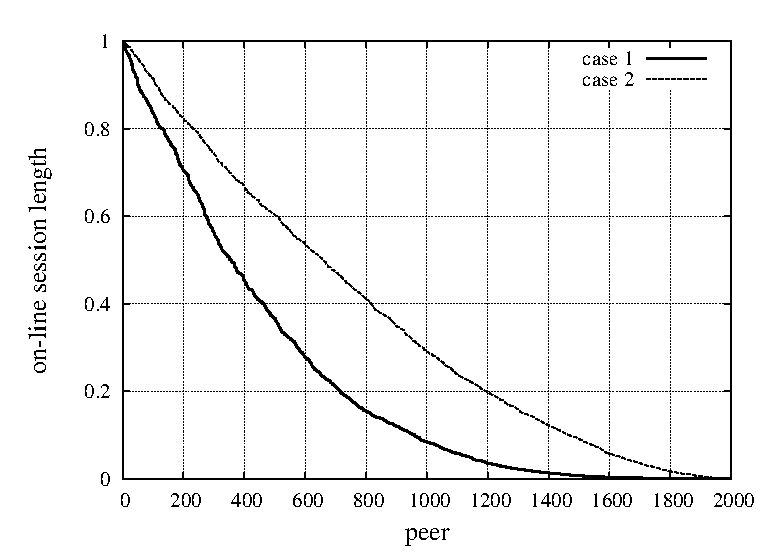
\includegraphics[width=0.99\columnwidth]{distribution.eps}\\
    \centering \small{(a) Distributions of on-line session lengths}
\end{minipage}
\begin{minipage}[t]{0.5\linewidth}
    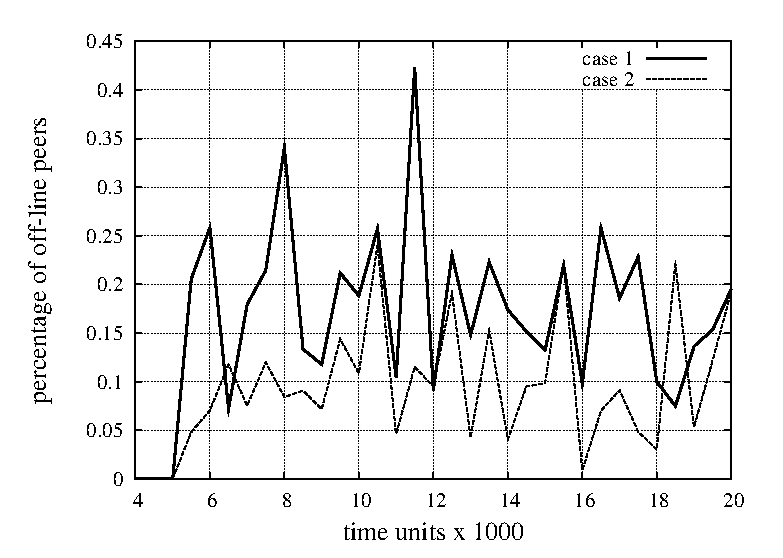
\includegraphics[width=0.99\columnwidth]{alive.eps}\\
     \centering \small{(b) Off-line peers over time}
\end{minipage}
\caption{Lifetime distributions} \label{fig:lifetime-distr}
\end{figure*}

We experimented with different lifetime distributions. Figure~\ref{fig:lifetime-distr}(a) illustrates two different on-line session length distributions. By definition, the more skewed the distribution is, the smaller the lifetimes of the most peers are. The first case in Figure~\ref{fig:lifetime-distr}(a) corresponds to a difficult scenario compared to the second case, since peers are on-line for shorter time periods and leave the network more often. Figure~\ref{fig:lifetime-distr}(b) presents the percentage of off-line peers as a function of time. In the first scenario the percentage of the peers that are logged-off reaches up to 42\% ($t=11.5K$), while in the second scenario the percentage of the logged-off peers every moment is kept under 25\%.

\subsection{Experimental Evaluation}
Figure~\ref{fig:rewiring}(a) presents clustering efficiency as a measure of  network organisation over time. The plots presented in the figure correspond to the two dynamic scenarios discussed in the previous section.

\begin{figure*}[t]
\begin{minipage}[t]{0.5\linewidth}
    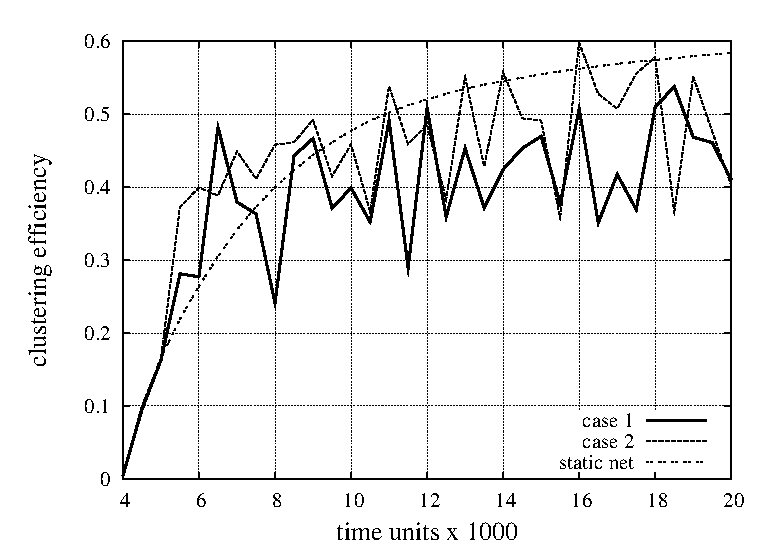
\includegraphics[width=0.99\columnwidth]{cE.eps}\\
    \centering \small{(a) Clustering efficiency}
\end{minipage}
\begin{minipage}[t]{0.5\linewidth}
    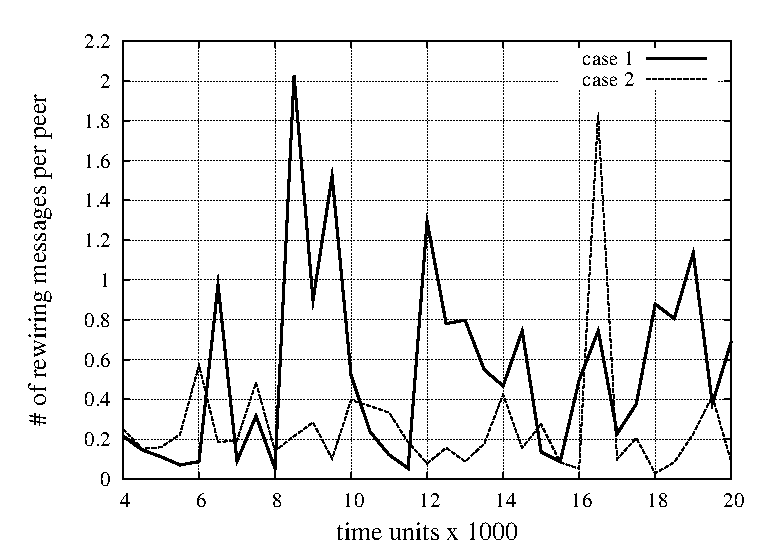
\includegraphics[width=0.99\columnwidth]{rew.eps}\\
     \centering \small{(b) Rewiring messages}
\end{minipage}
\caption{Rewiring effectiveness over time} \label{fig:rewiring}
\end{figure*}

Notice, by collating Figures~\ref{fig:rewiring}(a) and \ref{fig:lifetime-distr}(b), that clustering efficiency is narrowly related to the percentage of peers that are off-line; when the percentage of off-line peers increases clustering efficiency decreases, and vice versa.


\section{Conclusions}\label{sec:conclusion}
In this work, we studied the performance of SONs under churn, using established churn models that describe user behaviour in a realistic setting.

\bibliography{p2p-short}

\end{document}
